\section{Introduction}

%The cardiovascular system and its components have been vastly studied and a lot 
%of visualization techniques to study the heart or the arteries of the human body 
%have  been  proposed.  In  this  STAR  report,  you  need  to  conduct  a  survey  on 
%important  medical  visualization  applications  that  cover  the  topic  of 
%cardiovascular visualization, to propose a taxonomy of the existing applications, 
%and to provide an overview of yet-unaddressed or challenging topics.  

For diagnosis as well as for therapy planning it is crucial to understand the branching pattern and morphology of tree-like anatomical structures \cite{preim2013visual}.
Depending on the capturing technique we are confronted with 3D data that could have very high spacial or temporal resolution. The visual analysis of this static or dynamic data is a challenging task.

\begin{figure}[h]
	\centering
	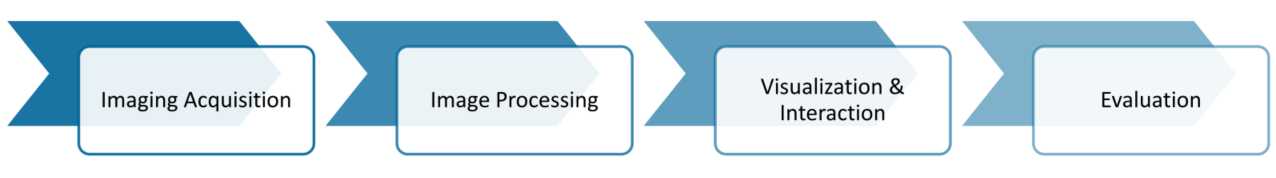
\includegraphics[width=0.45\textwidth]{MedicalVisualizationPipeline.png} \\
	\caption{Medical visualization pipeline.}
	%\cite{volkau2005geometric}
	\label{fig:MedicalVisualizationPipeline}
\end{figure}

The medical visualization pipeline shown in figure \ref{fig:MedicalVisualizationPipeline} serves as orientation how vascular structures are visualized. We are focusing on 3D image processing and visualization. The interested reader will find a complete survey of the whole pipeline for instance in \cite{preim2013visual}. 

Our goal here is to describe recent methods to visualize vascular structures. Our initial interest is on how to separate these structures from background data. Direct volume rendering techniques can be used to visualize this enhanced and visually separated data. If a more concrete separation is necessary, surface visualization techniques may be preferable, which involve segmentation and centerline extraction. 

Visualization techniques are spilt into \emph{model-based} and \emph{model-free} approaches. 
Model-based mesh generation follows some more restrictive assumptions about the vascular structure whereas model-free methods such as direct volume rendering tries to capture as much original information as possible. Model-based techniques are often used for treatment planning and basic anatomical overview, whereas model-free methods are required for precise diagnostics.

% \subsection{Taxonomy}

